%-------------------------------------------------------------------------------
% File: database.tex
%       Part of StockSim project documentation.
%       See main.tex for further information.
%-------------------------------------------------------------------------------
\chapter{Database}

The dataset is composd by 8236 stocks from the US stock market, along with
their general informations and historical data; the application also need to store 
users' and admins' credential, personal informationof users, composition and details of
each user's porfolio.
We decided to use a column database for the storage of historical data; those 
informations represent around the 92.5\%\ of our dataset and they are going to grow very fast
during time; aggaregation and financial analytics on these volumes of data will perform
better in a colum database where data storage is design to optimize this type of operations;
We decided to store every other information in a document database, in order to exploit the
schemaless property for save memory; information frequently needed toghether will be stored 
in the same document and indexes are created to speedup linking beetween documents; 


\section{Dataset}


\subsection{Yahoo! Finance}

\subsection{NasdaqTrader}

\section{MongoDB}
"MongoDB is a general purpose, document-based, distributed database built 
for modern application developers and for the cloud era." Taken from www.mongodb.com.
MongoDB is a very famous document database with a great support for cloud operations, witch 
will improve the avaliability of our application. It also suport a lot of analytics functions
and the creation of custom indexes in order to speedup read operations.
In order to orgnize data ina a meaningfull and memery-optimal way, we opted for this structure:

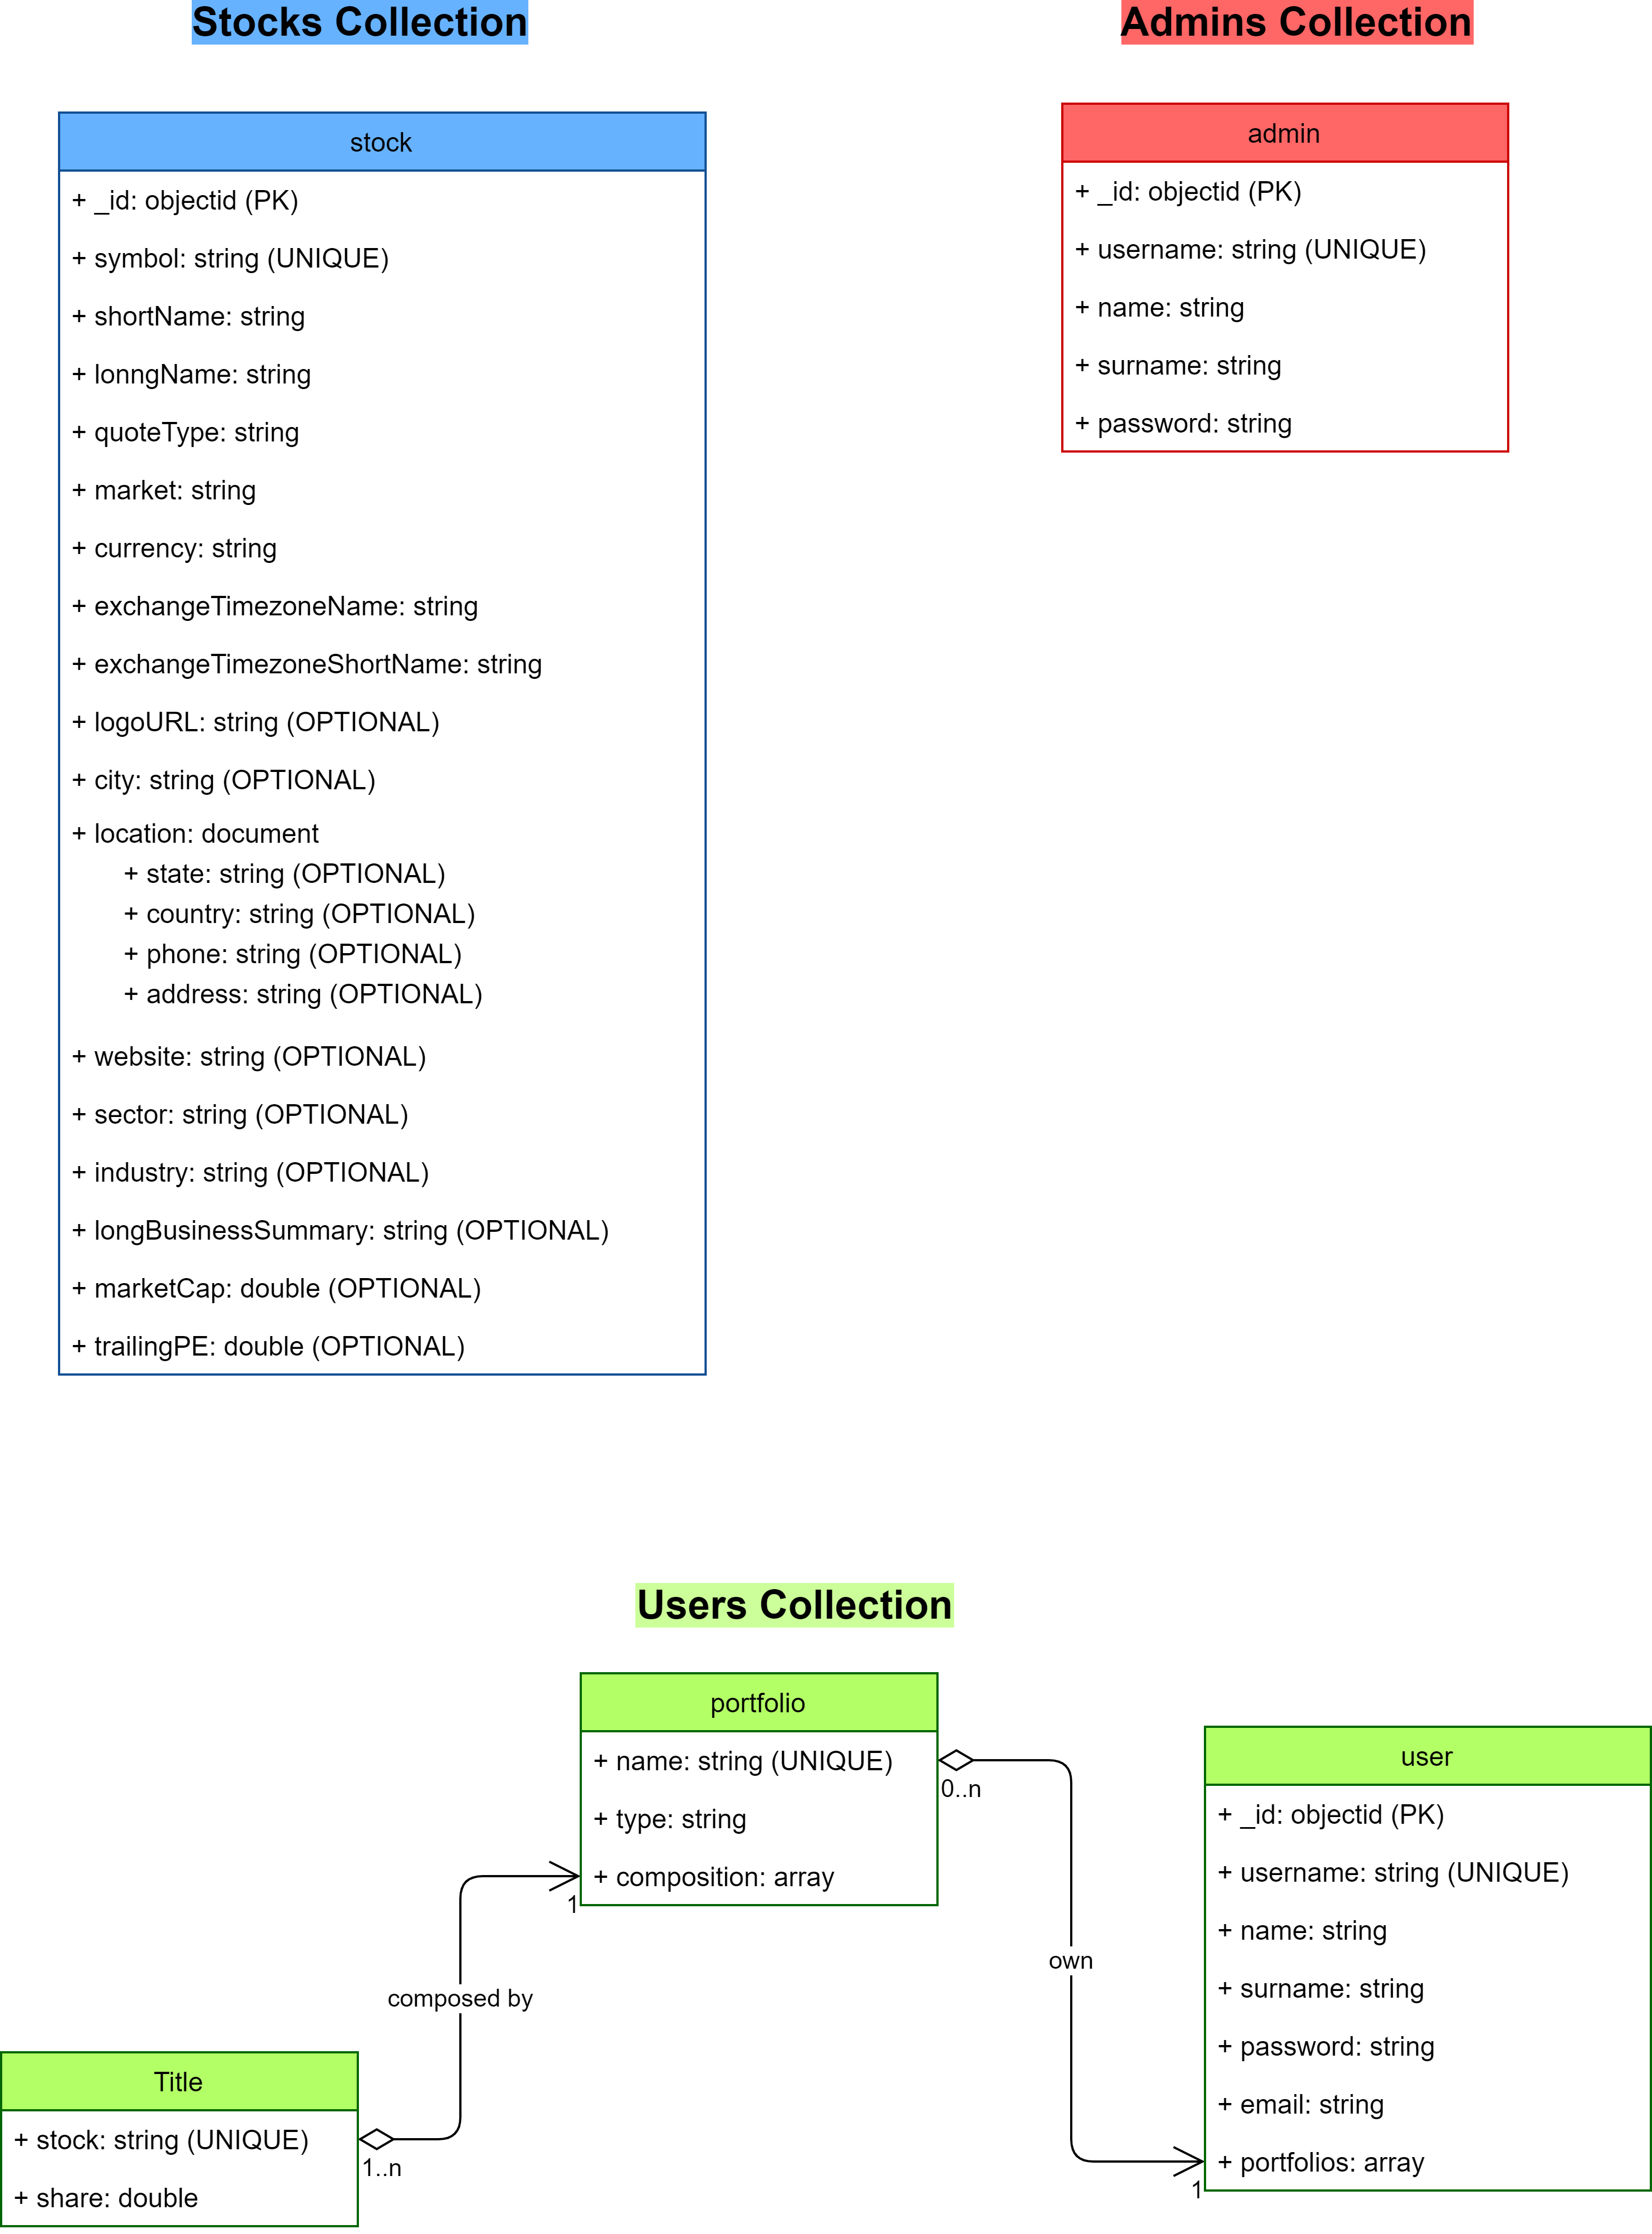
\includegraphics[scale=0.15]{img/mongoDB_schema.png}

This scheme is composed by 3 collections: \textbf{stocks}, \textbf{users}, \textbf{admins};
\begin{itemize}
    \item
The stocks collection contains one document for each stock; inside this document are stored 
all the general information about the stock, wich is identified by the attribute SYMBOL;
some basic information are always presents, while others are missing for some stocks; we decided 
to keep these last type of informations where possible, exploiting the schemaless property of
the documentat databse;
    \item
The users collection contains one docuemt for each user regitered on the application; for every
user login credentials are stored, along with few personal information; for every user is 
also stored an array of documents named PORFOLIOS: this array contains the porfolios of the user.
Each portfolio has a scheme, witch include an array of TITLEs, named COMPOSITION, witch represent
the settlement of the portfolio itsef. This nested structure it's been preferred from splittin
data in different collections, because all the information of a user, including his portfolios, 
are frequently needed toghether; on the other hand, there aren't such operations that involve
porfolios owneds by different users.
    \item 
The admins collection contains the admins login credentials toghether with few personal
informations about them; we decided to crerate a separated collection for administators 
to improve the security of the administration features: in this way is impossible to inject
administration privileges throw the login command.
\end{itemize}
\subsection{Aggregations}
One of the main features of own application is the possibility to choose some stocks from
the market and combine them in to a portfolio. When a user is looking for a stock, he want to
know statistic about \textbf{industies} and \textbf{sectors}, along with classification by 
\textbf{level of capitalization} and  \textbf{PE ratio}; in ordewr to do so, we will provide
these aggregation pipelines:
\begin{itemize}
    \item the total market capitalization of each sector
    \item the total market capitalization of each industry
    \item the total market capitalization of stocks coming from the same country
    \item the avarage PE ratio of stocks working in the same sectors
    \item the avarage PE ratio of stocks working in the same industry
    \item the avarage PE ratio of stocks coming from the same country
    \item the avarage PE ratio of stocks beeing in a specific range of market capitalization
\end{itemize}
\subsection{Indexes}
In order to speeup read operation in the document database, 
we decided to introduce some custom indexes:
\begin{itemize}
    \item a REGULAR and UNIQUE index on the attribute \textbf{symbol} in the collection stocks;
    \item a REGULAR index on the attribute \textbf{marketCAP} in the collection stocks;
    \item a REGULAR index on the attribute \textbf{trailingPE} in the collection stocks;
    \item a REGULAR index on the attribute \textbf{sector} in the collection stocks;
    \item a REGULAR index on the attribute \textbf{industry} in the collection stocks;
    \item a REGULAR index on the attribute \textbf{country} in the collection stocks;
    \item a REGULAR and UNIQUE index on the attribute \textbf{username} in the collection users;
\end{itemize}
We provide some statistic that endorse our idexes choises

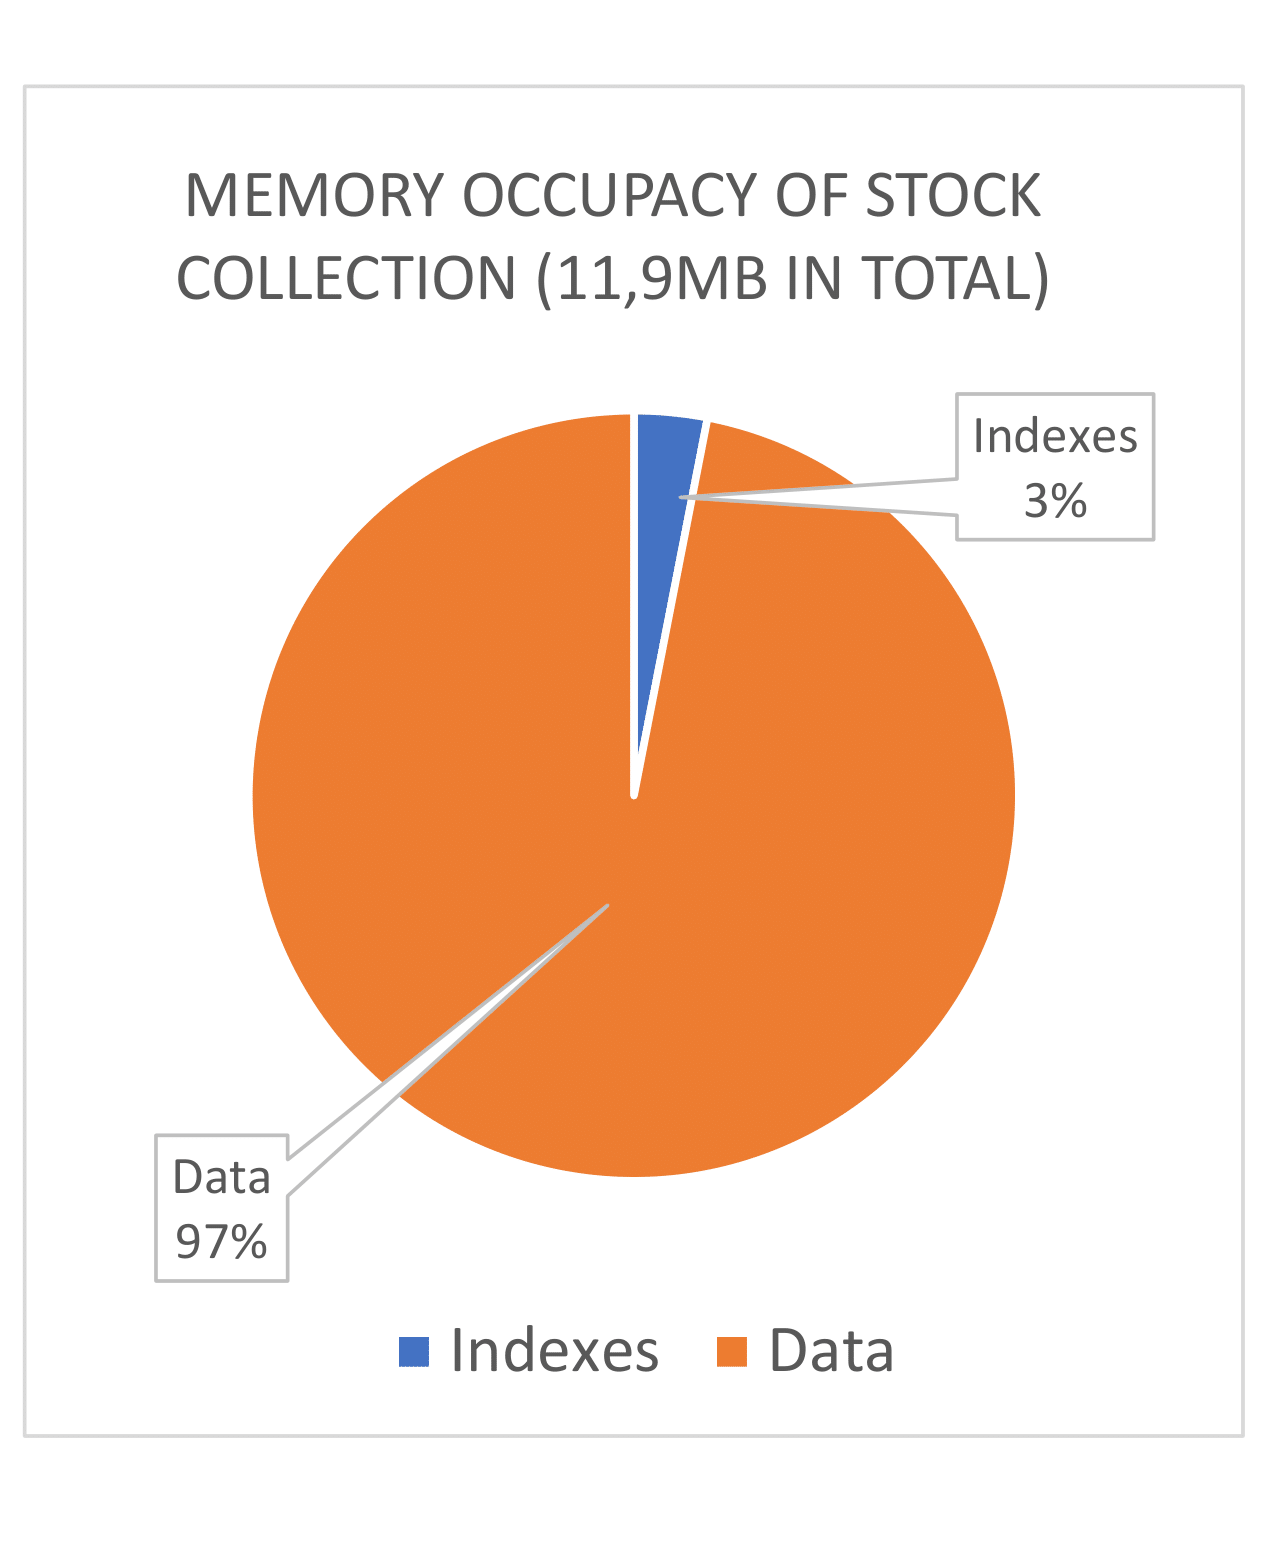
\includegraphics[scale=0.07]{img/memory_mongo.png}
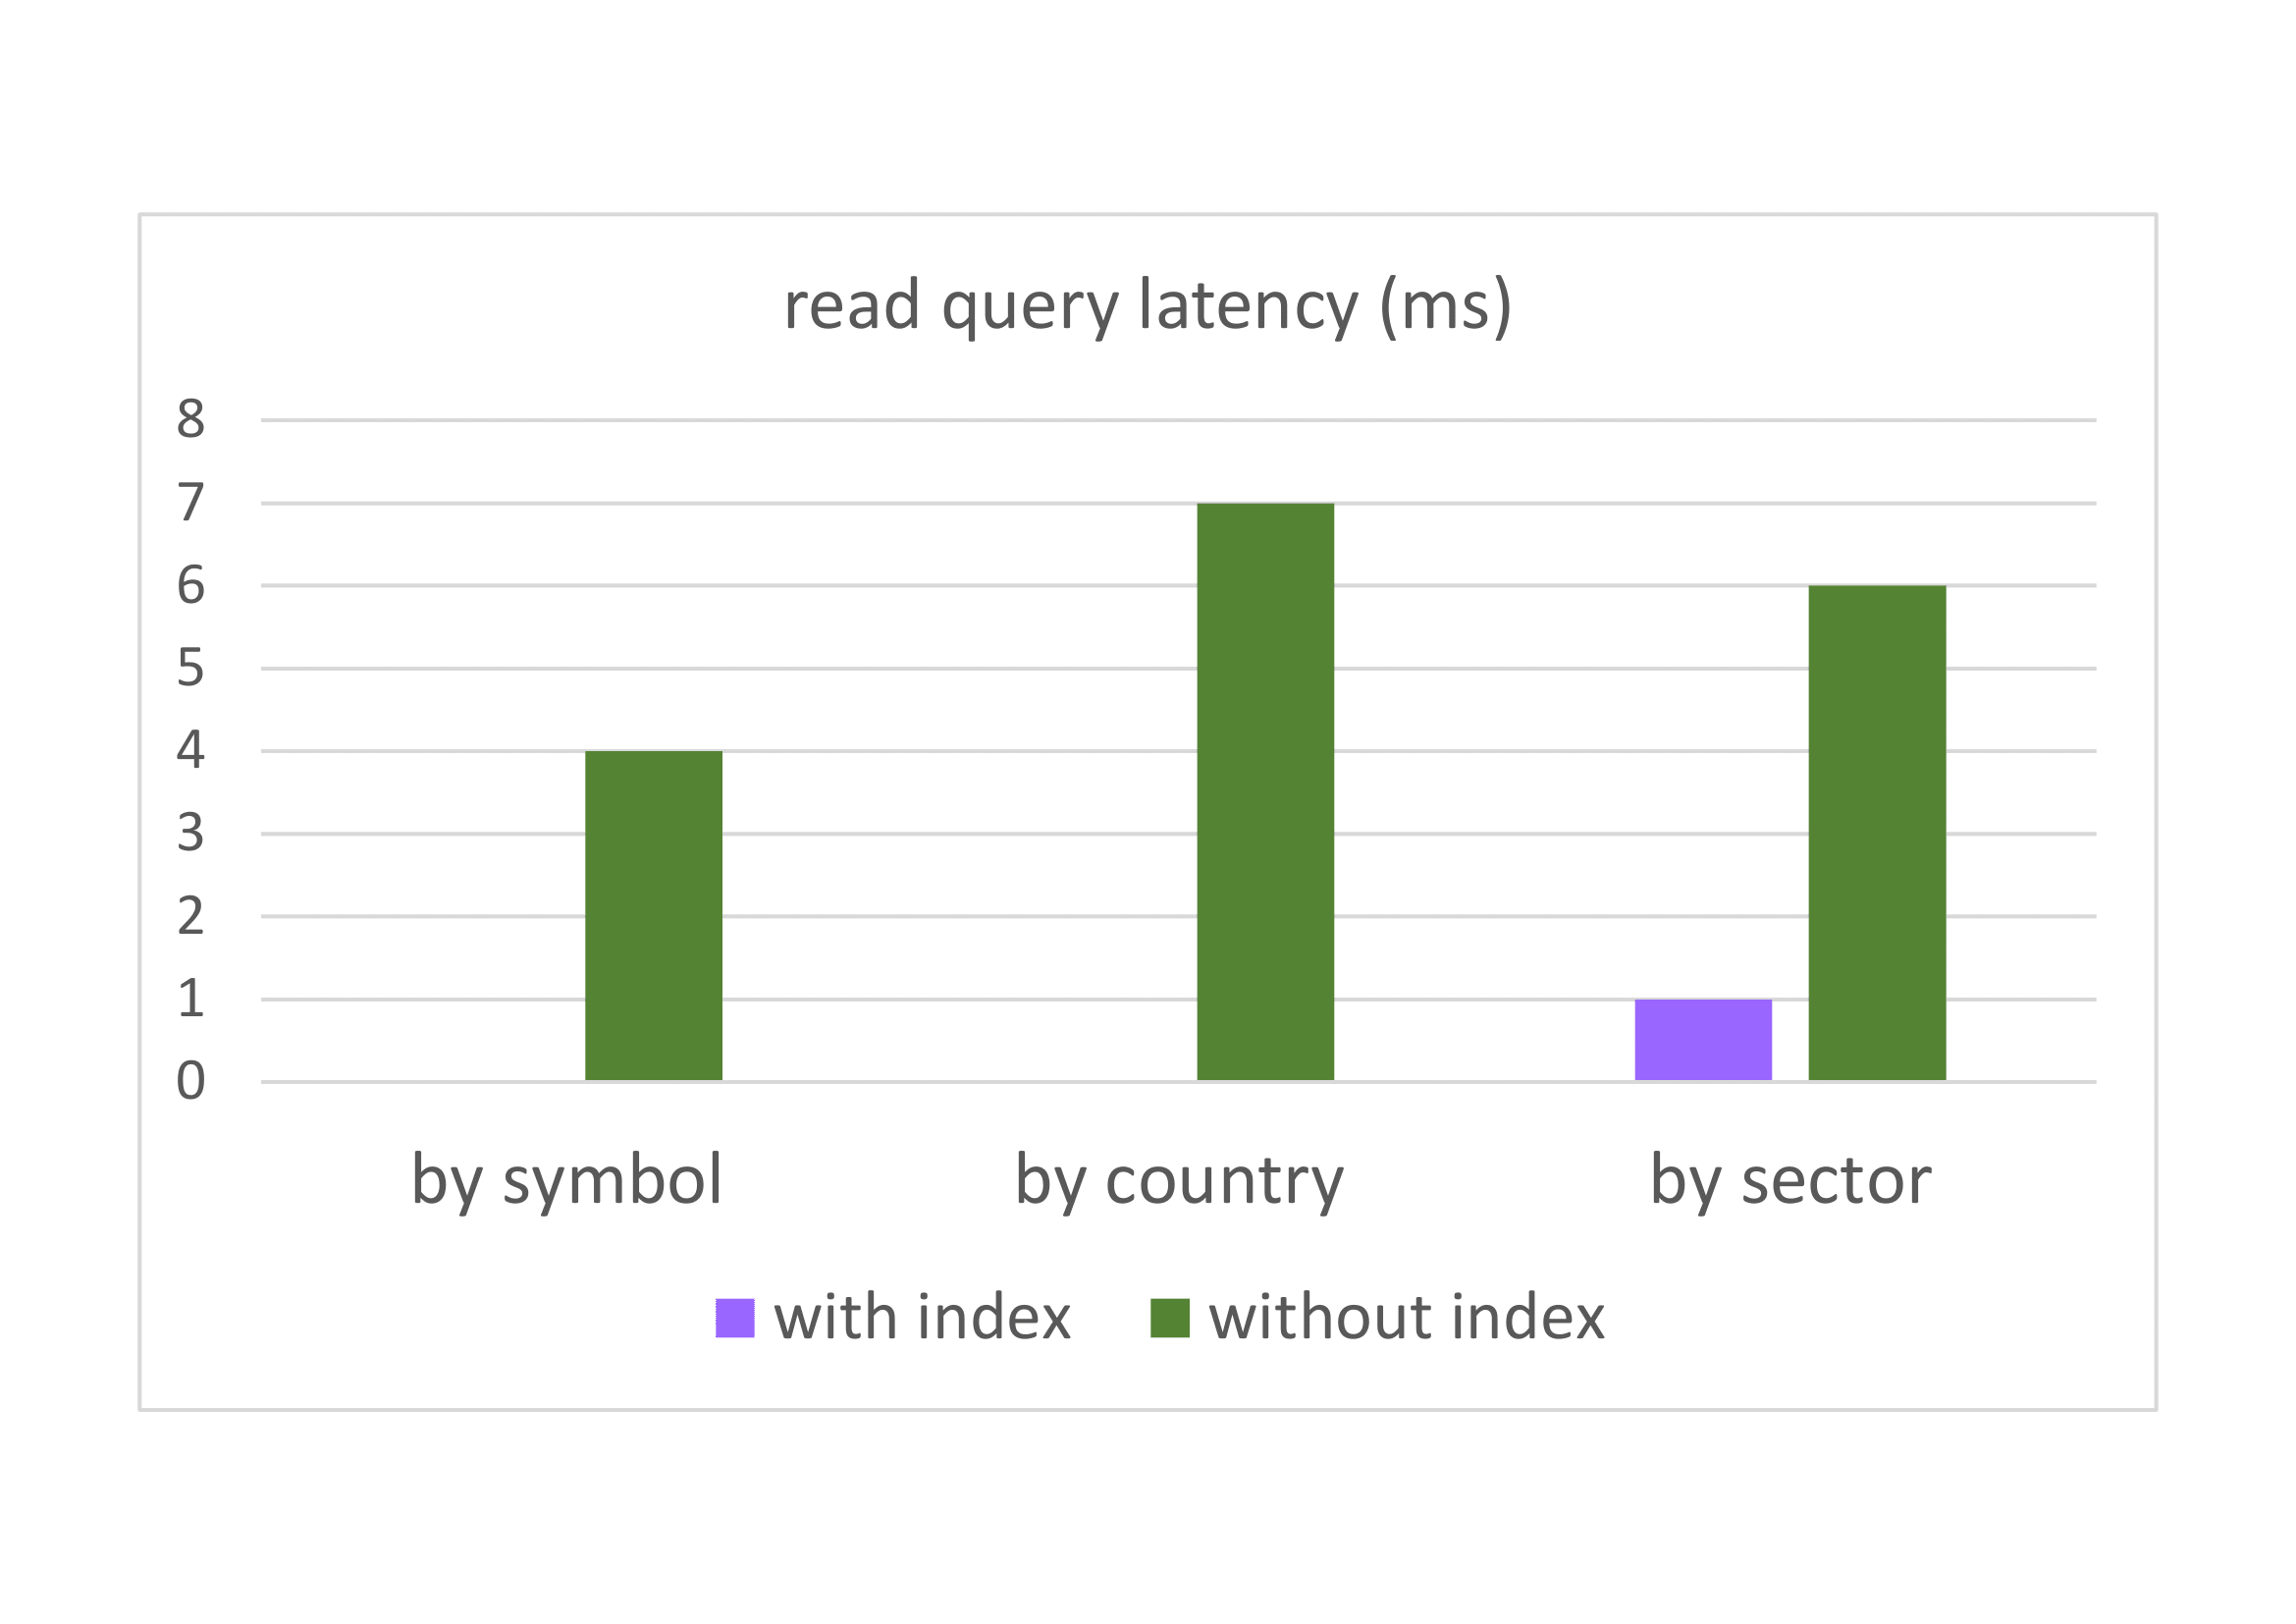
\includegraphics[scale=0.07]{img/latency_mongo.png}

Analog results can be found about the username index in the users collection.

\section{Apache Cassandra}

\subsection{Aggregations}
\subsection{Indexes}

\section{Sharding and Replicas}

\section{Apache Cassandra vs MongoDB}
